\chapter{Results}
\label{chap:results}



\section{Captured images}
16 fps 10 bit synchonized stereo images!


\pagebreak
% \begin{figure}[H]
%     \centering
%     \begin{tabular}[b]{cc}
%         \subcaptionbox{Original frame.}{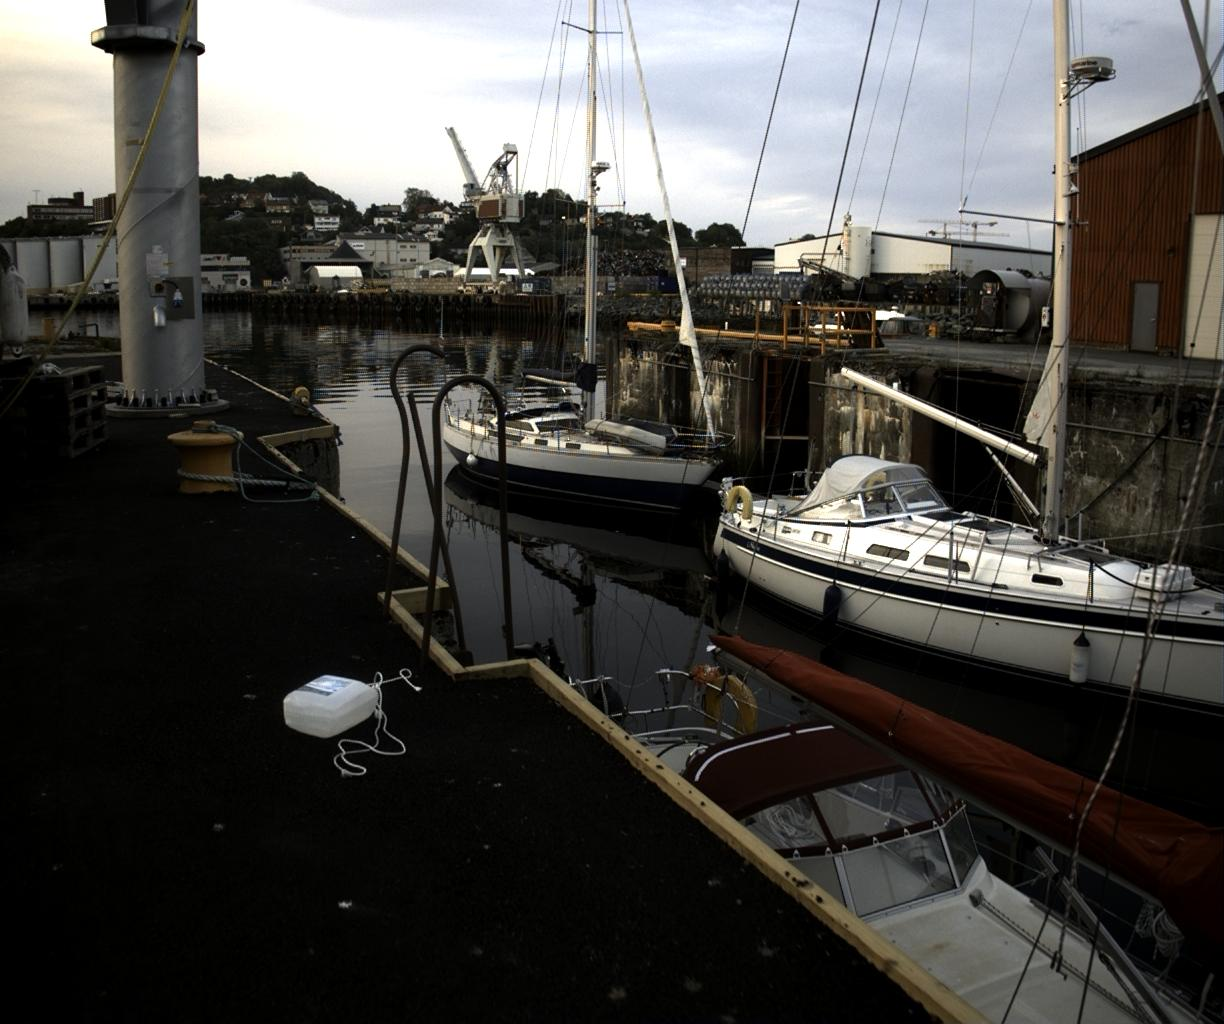
\includegraphics[width=.9\textwidth]{figures/pictures/regular_right_96.jpeg}} \\
%         \subcaptionbox{Original frame subtracted from decompressed frame.}{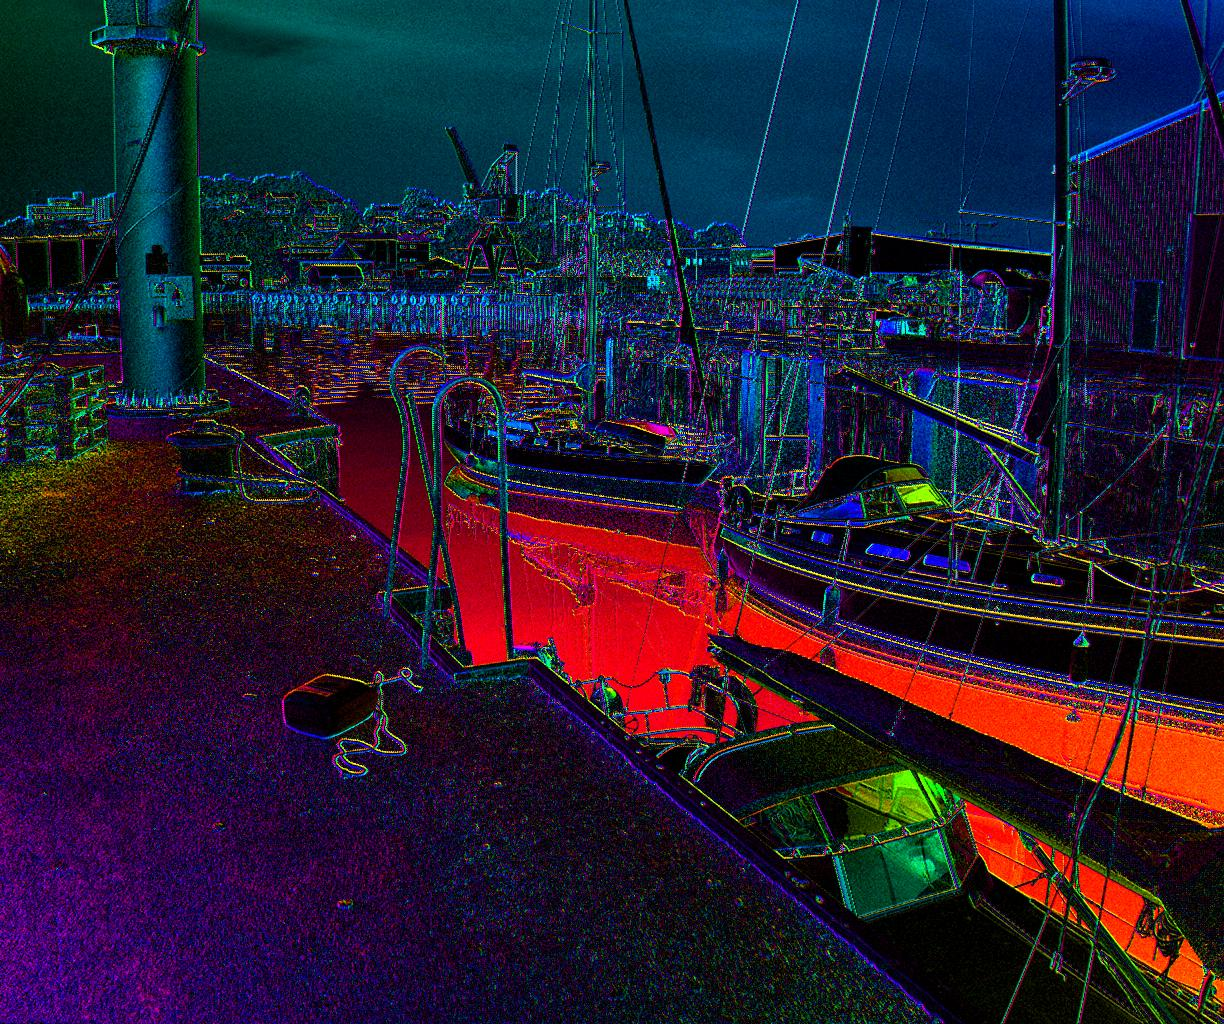
\includegraphics[width=.9\textwidth]{figures/pictures/aolp_right_96.jpeg}}
%     \end{tabular}
%     \caption{Original frame and compression error revealing use of wrong color profile as brigh regions are too dark and dark regions are too bright.}
% \end{figure}
\begin{figure}[H]
    \centering
    \subcaptionbox{Mean image.\label{fig:normal_img}}{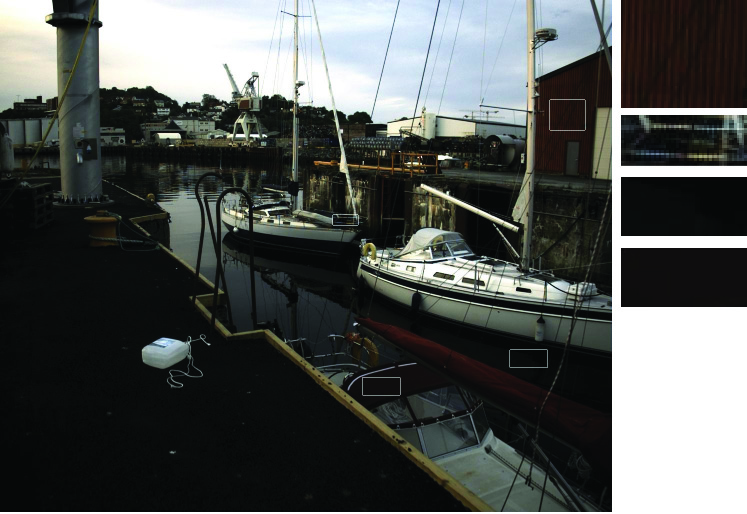
\includegraphics[width=\textwidth]{figures/pictures/result_rgb.jpg}}
    \subcaptionbox{HSV visualization of polarization data where the angle of polarization is encoded as hue and degree of polarization is encoded as value.}{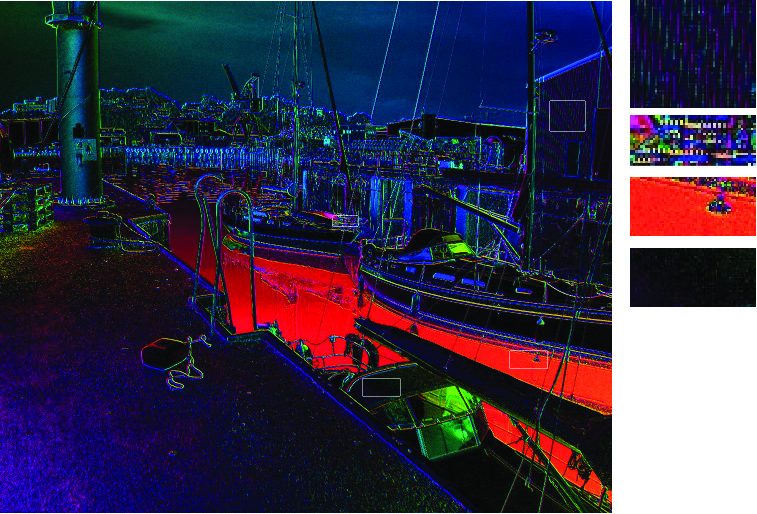
\includegraphics[width=\textwidth]{figures/pictures/result_pol.jpg}}
    \caption{Right image \#1536 with, zoomed in regions of interest.}
\end{figure}

\begin{figure}[H]
    \centering
    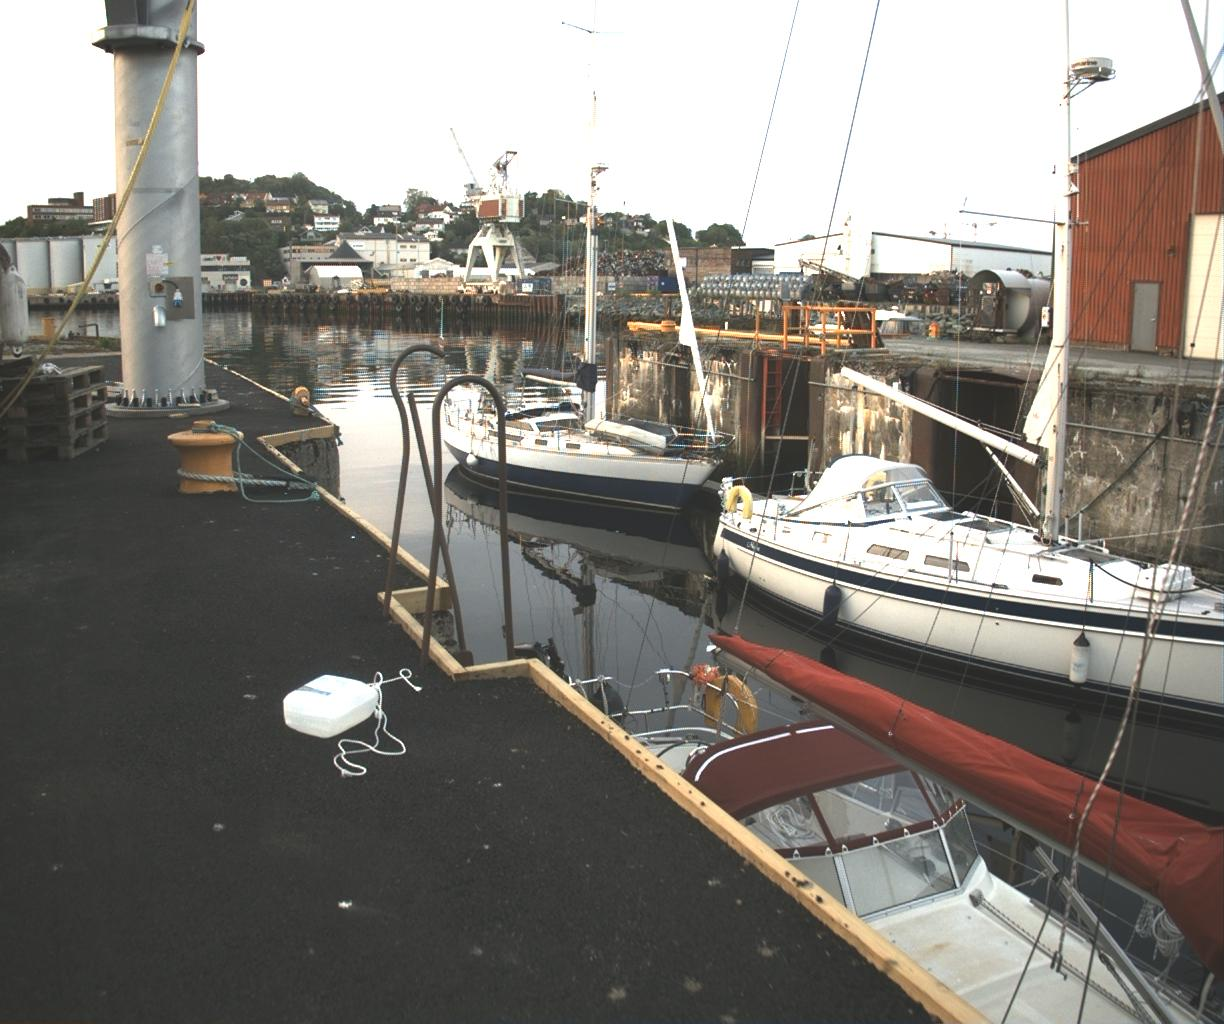
\includegraphics[width=.8\textwidth]{figures/pictures/gained_right_96.jpeg}
    \caption{Image showing how dark areas contain a lot of information thanks to 10-bit depth.
        The image is the same as in Figure \ref{fig:normal_img}, but with brightness increased.}
    \label{fig:gained_image}
\end{figure}

\begin{figure}[H]
    \centering
    \subcaptionbox{Mean image.\label{fig:normal_img}}{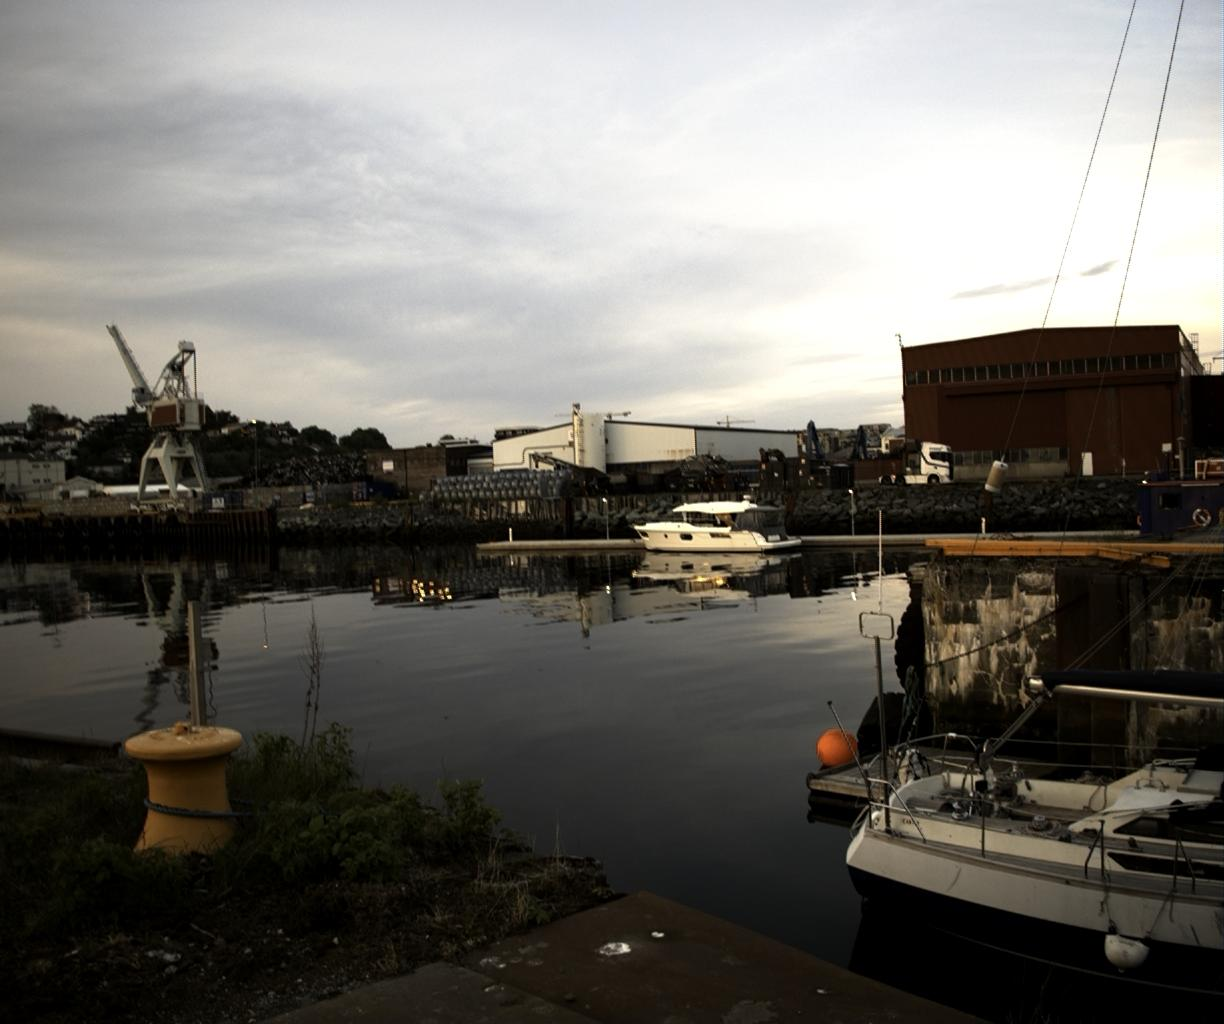
\includegraphics[width=.9\textwidth]{figures/pictures/regular_left_124.jpeg}}
    \subcaptionbox{HSV visualization.}{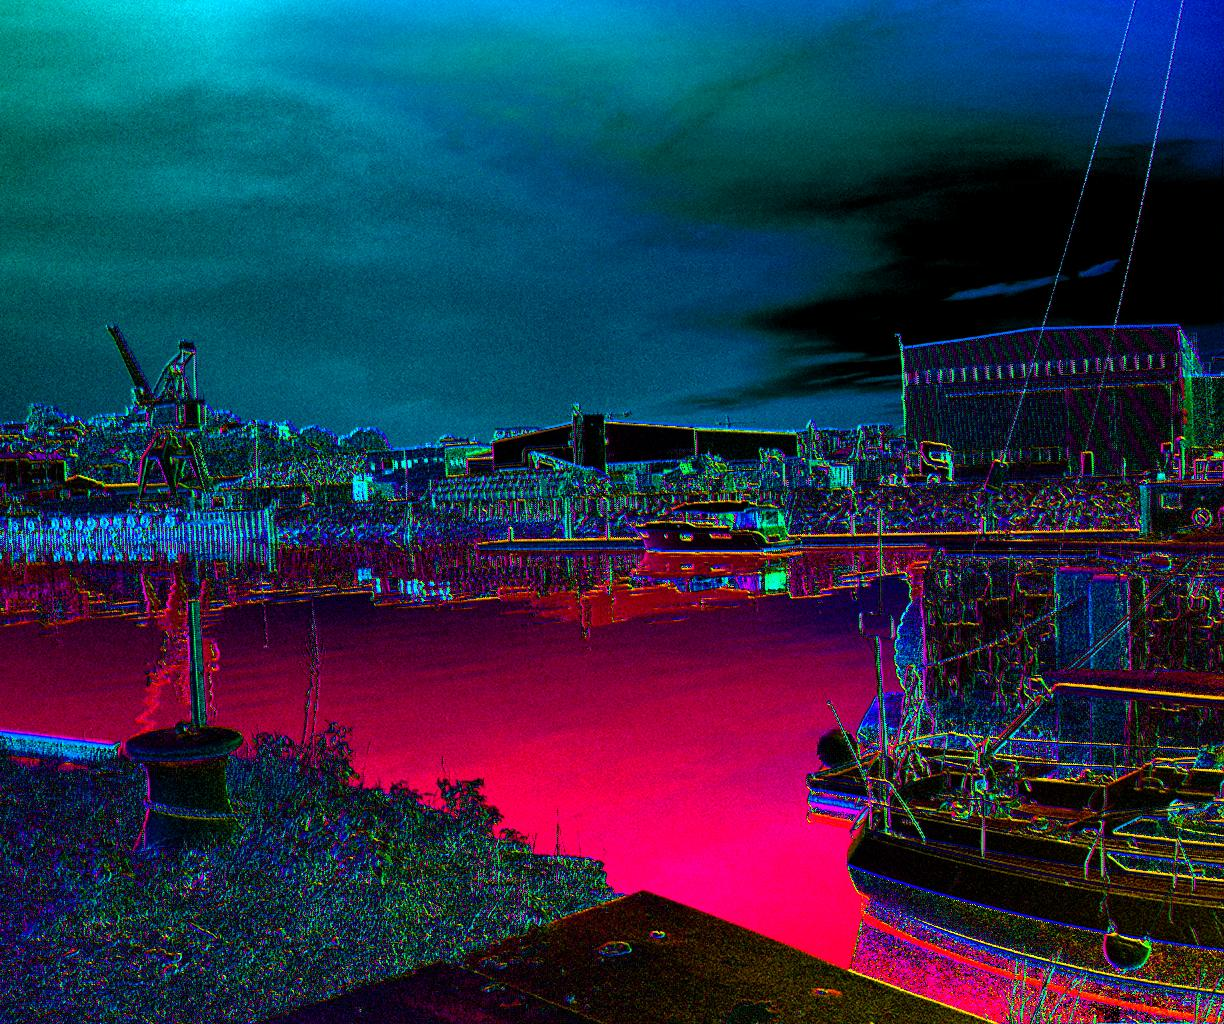
\includegraphics[width=.9\textwidth]{figures/pictures/aolp_left_124.jpeg}}
    \caption{Left image \#1984}
\end{figure}
\begin{figure}[H]
    \centering
    \subcaptionbox{Mean image.\label{fig:normal_img}}{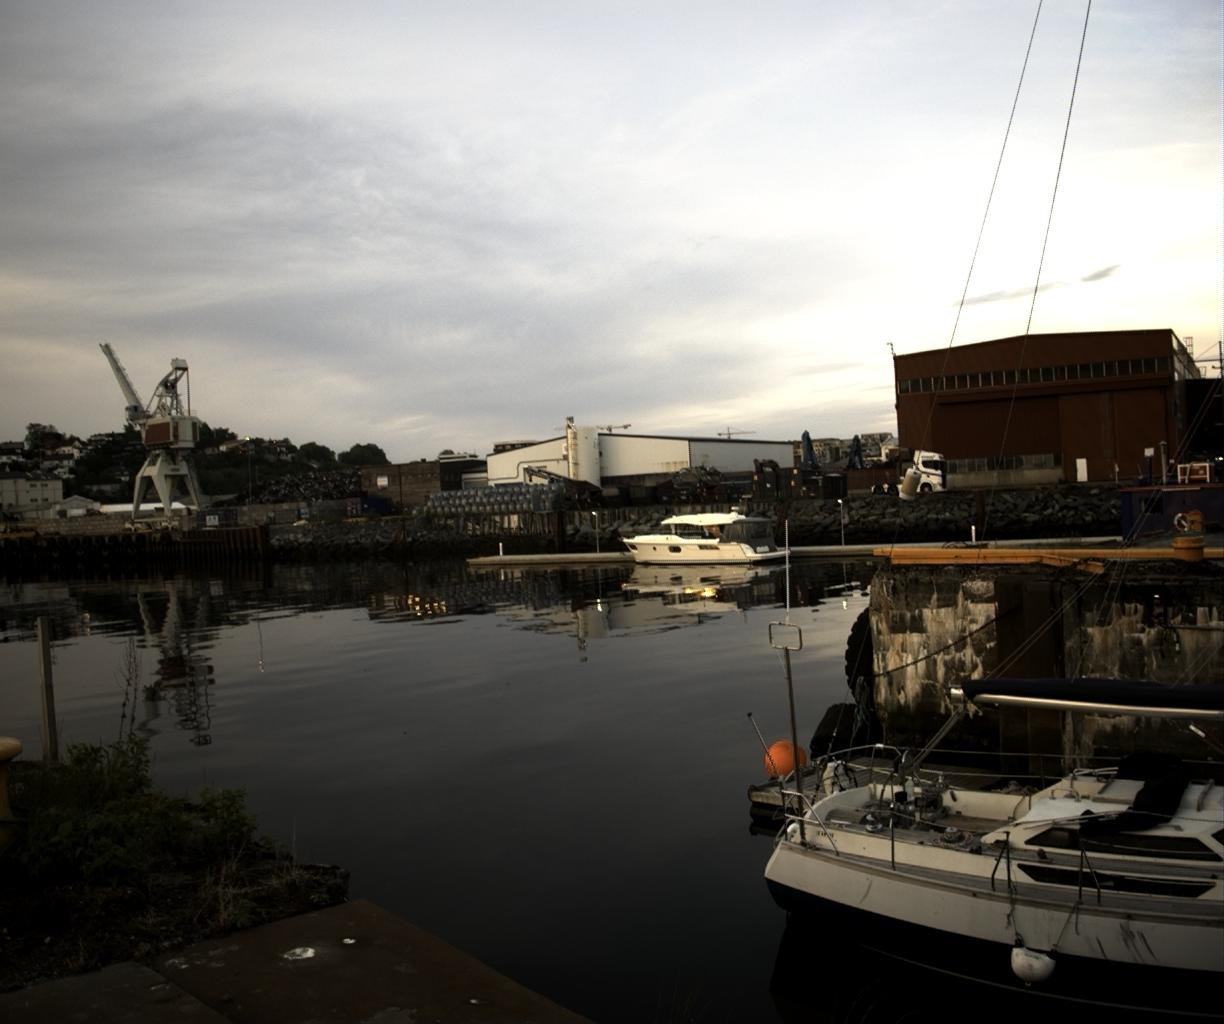
\includegraphics[width=.9\textwidth]{figures/pictures/regular_right_124.jpeg}}
    \subcaptionbox{HSV visualization.}{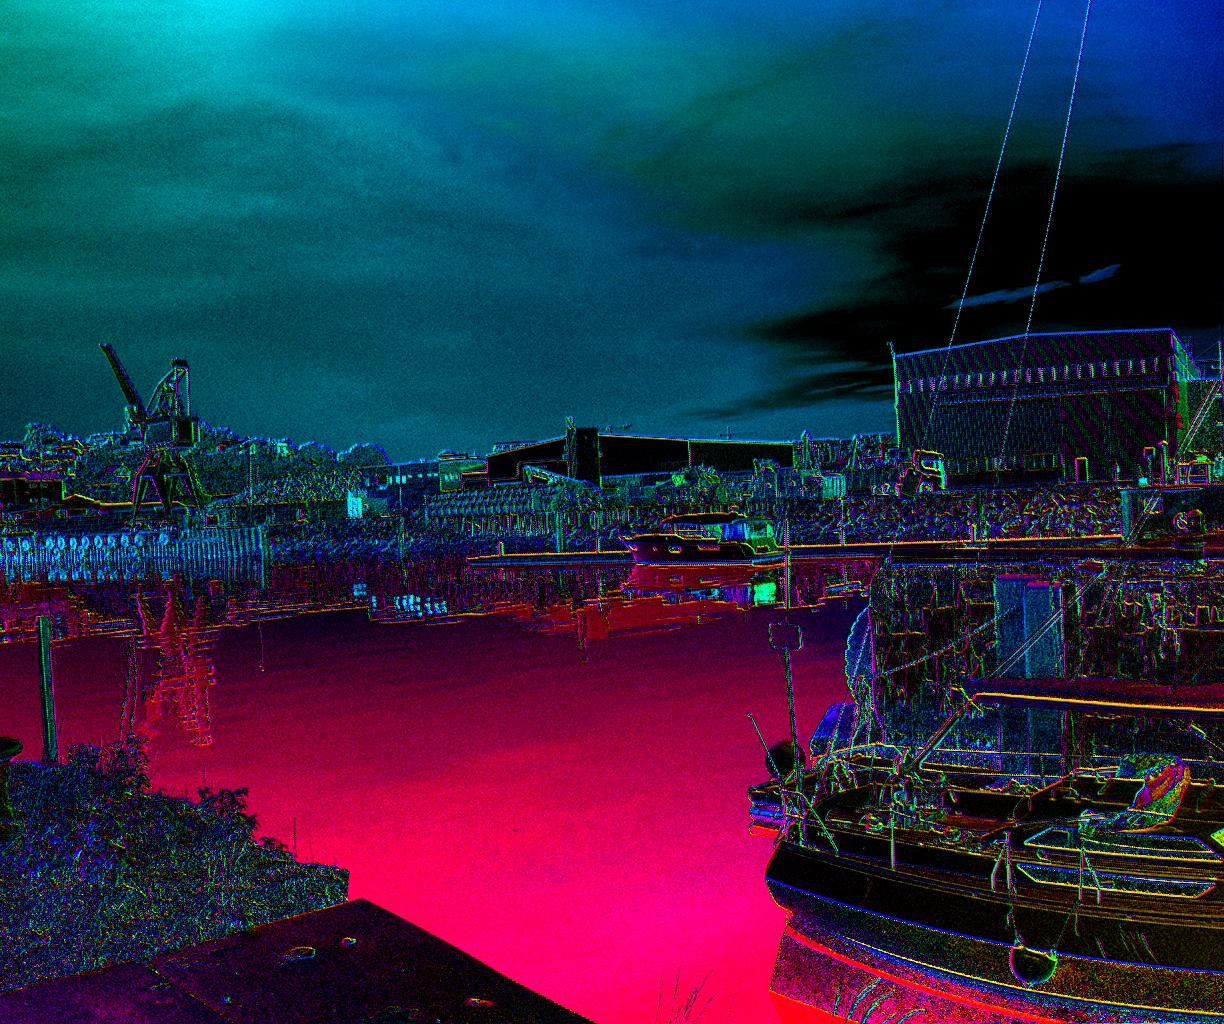
\includegraphics[width=.9\textwidth]{figures/pictures/aolp_right_124.jpeg}}
    \caption{Right image \#1984}
\end{figure}




\section{Debayering}
The custom



\section{Compression}



The most efficient video compression method the \jx support is \gls{h265}.

\subsection{Testing method}
To get a rough estiamte of the expected compression performance of the \gls{h265} encoder, a small test was performed.






Without performing any tuning of the compression parameters, the pipeline coppresses the video stream by 75\% on average.


Less than 0.6\% relative error on average at with a 75\% space saving compression ratio.
Possible to acheive better and trade of error for compression ratio.

\subsection{HSV}
Another color representation that is relevant in this \master is \gls{hsv}.
This format is what is usually used when selecting color in a color picker.
A usefull property of this format is that it can be used to easily visualize